\documentclass{article}
\usepackage[top=0.75in,bottom=0.75in,left=0.8in,right=0.8in]{geometry}
\usepackage{enumerate,xspace,amsmath,amsfonts,amsthm,graphicx,hyperref}

\newcommand{\solution}[1]{\textbf{Solution:} #1}
\newcommand{\cut}[1]{\ensuremath{\mathnormal{}{cut}(#1)}}
\newcommand{\calg}{\ensuremath{{\cal G}}\xspace}
\newcommand{\calo}{\ensuremath{{\cal O}}\xspace}
\newcommand{\opt}[1]{\ensuremath{\text{OPT}(#1)}}
\newcommand{\length}[1]{\ensuremath{\overline{#1}}}

% macro for a set. extra pair of braces inside \ensuremath to ensure
% the set is typseset in one line.
\newcommand{\set}[1]{\ensuremath{{\{#1\}}}}

\newcommand{\R}{\mathbb{R}}
\newcommand{\C}{\mathbb{C}}
\newcommand{\F}{\mathbb{F}}
\newcommand{\N}{\mathbb{N}}
\newcommand{\Z}{\mathbb{Z}}
\newcommand{\Q}{\mathbb{Q}}
\newcommand{\cL}{\mathcal{L}}
\newcommand{\cB}{\mathcal{B}}
\newcommand{\cM}{\mathcal{M}}
\newcommand{\cC}{\mathcal{C}}
\newcommand{\cE}{\mathcal{E}}
\newcommand{\cV}{\mathcal{V}}
\newcommand{\cP}{\mathcal{P}}
\newcommand{\cU}{\mathcal{U}}

\theoremstyle{definition}
\newtheorem{exmp}{Example}

\renewcommand{\baselinestretch}{1.3} 
\begin{document}
\thispagestyle{empty}

\begin{center}{\bf Tacoma Narrows Bridge}\end{center}

On July 1, 1940, a bridge spanning the Tacoma Narrows opened
to great celebration. It dramatically shortened the trip from Seattle
to the Kitsap Peninsula. It was an elegant suspension bridge, a mile
long (third longest in the US at the time) but just 39 feet across.
Through the summer and early fall, drivers noticed that it tended to
oscillate vertically, quite dramatically. 

During the first fall storm, on November 7, 1940, with steady winds
above 40 mph, the bridge began to exhibit different behavior. It
{\it twisted}, part of one edge rising while the opposing edge fell, and then
the reverse. At 10:00 AM the bridge was closed. The torsional oscillations continued to grow in amplitude, until, at just after 11:00, the
central span of the bridge collapsed and fell into the water below. One
car was lost.

Why did this collapse occur? Were the earlier oscillations a warning
sign? Many differential equations textbooks announce that this is an
example of {\it resonance}: the gusts of wind just happened to match the
natural frequency of the bridge.
\begin{figure}[!htb]
\minipage{0.33\textwidth}
  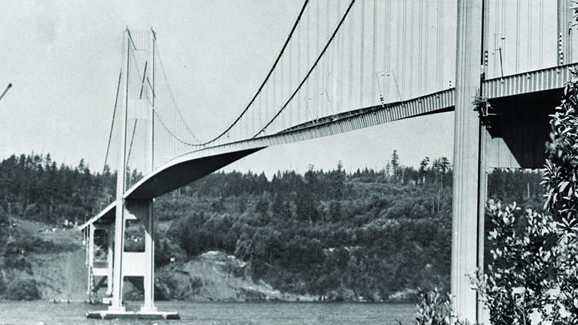
\includegraphics[width=\linewidth]{tac01}
\endminipage\hfill
\minipage{0.33\textwidth}
  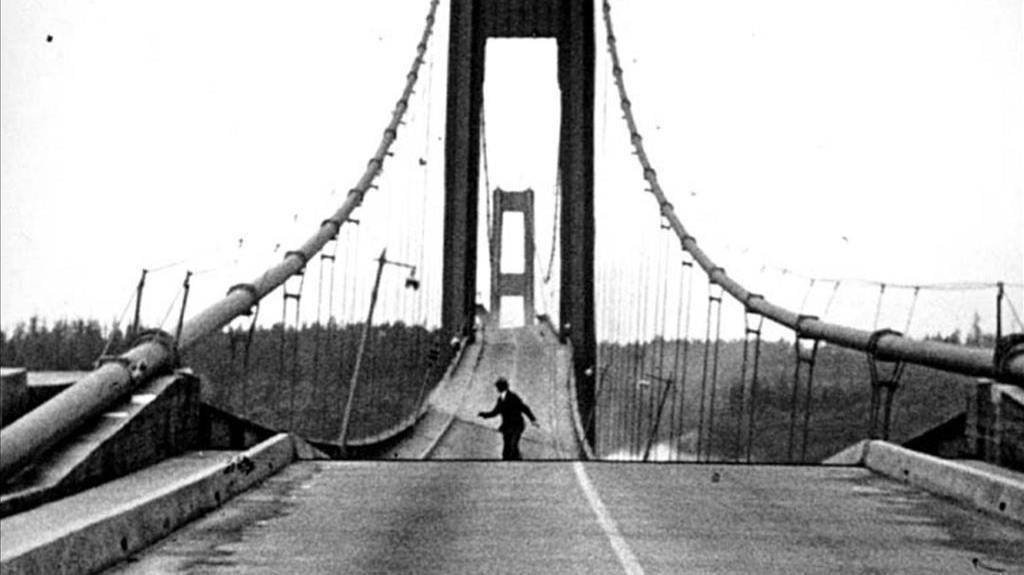
\includegraphics[width=\linewidth]{tac02}
\endminipage\hfill
\minipage{0.33\textwidth}%
  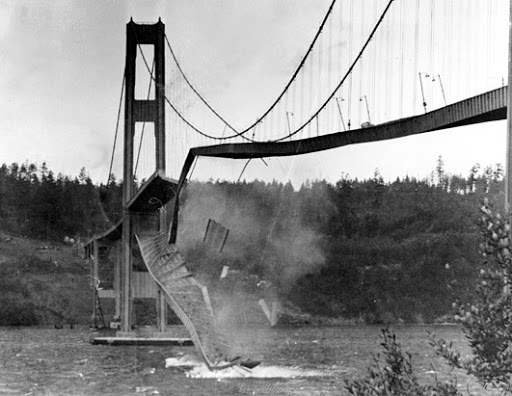
\includegraphics[width=\linewidth]{tac03}
\endminipage
\end{figure}

\noindent{\bf Models:}
Let the vertical deflection
(positive direction downward) of the slice of the roadbed denoted by $y(t)$, where $t$ represents time, and $y=0$ represents the equilibrium position of the road. 

\begin{enumerate}
\item
Here are three simplified second order differential equations that model the situations of the Tacoma Bridge. Assume that at the initial time, the displacement of the bridge $y(0)=0$, and the velocity of the bridge $y'(0)=0.1$,  so that the roadbed
starts in the equilibrium position with a small downward velocity. For each of the following equations, find the solution to the IVP with these initial conditions. Graph the solutions, and describe the short-term and long-term behavior of the solutions.
\begin{enumerate}
\item {\bf Without force.} $\dfrac{d^2y}{dt^2} + 4y = 0$.
\item {\bf With periodic forcing.} $\dfrac{d^2y}{dt^2} + 4y = \cos(t)$.
\item {\bf In resonance.} $\dfrac{d^2y}{dt^2} + 4y = \cos(2t)$.
\end{enumerate}

\item Perfect coincidences are rare in nature: it's very unlikely for the wind frequency to exactly equal the natural frequency of the bridge.
\begin{enumerate}
\item Before solving, what do you expect to happen to the solution of the IVP with same initial conditions and equation $\dfrac{d^2y}{dt^2} + 4y = \cos(1.9 t)$? 
\item Graph the solution to the IVP described in the last part, and describe the short-term and long-term behavior of the solutions.
\item Repeat the last two questions for $\dfrac{d^2y}{dt^2} + 4y = \cos(1.99 t)$.
\item What happens in the limit with the same IVP with $\dfrac{d^2y}{dt^2} + 4y = \cos(\alpha t)$ as $\alpha \to 2$?
\end{enumerate}
\end{enumerate}


\end{document}
\begin{verbatim}
\end{verbatim}